\chapter{Integration of Slow Control Channels in LIGO CDS}
\label{c:slow-controls-integration}

\section{The LIGO CDS system}
The \gls{CDS} system designed for use in \gls{LIGO} and used for the practical experiments in Chapters \note{X, Y, Z} provides high-speed, low-noise analogue-to-digital and digital-to-analogue converters (\gls{ADC}s and \gls{DAC}s, respectively) to send signals between the experimental hardware and the software-defined controls. The software-defined controls run within a real-time Linux kernel, allowing for deterministic operation, and the channel infrastructure is built on top of the widely used open-source \emph{\gls{EPICS}} system. While \gls{CDS}'s inputs and outputs are well suited to the measurement and control of key sensors and actuators within a low-noise experiment, they are also expensive. Each input or output channel consists of various integrated circuits and filters, all of which must be carefully chosen to minimise noise which can potentially contaminate the sensitivity of the system, along with power supply components, specialised connectors and rack infrastructure; this leads to an expense per channel of roughly \checkme{\pounds600}.

\section{EPICS and CDS}
Industrial-style control is not uncommon in large physics experiments such as \gls{LIGO}. Originally designed for the Advanced Photon Source particle physics experiment at Argonne National Laboratory, Chicago, USA, the \gls{EPICS} system provides the ability to define an arbitrary number of channels for the purposes of control. The \gls{CDS} system uses \gls{EPICS} to handle its control infrastructure.

\subsection{Input/output controllers}
One of the key advantages of this system is that the channels may be defined across any number of separate input/output controllers (\emph{IOC}s), which may be on separate, remote servers. This is useful from the point of view of large experiments, where to minimise transmission noise pick-up (see \ref{sec:signal-and-noise-paths}) controllers are situated close to devices to be controlled. At the Advanced LIGO facilities, for example, the end stations are separated from the main building by \SI{4}{\kilo\meter}, and so transmission noise to and from the main building would be significant. Instead, \gls{IOC}s are present within each end station, communicating with the master control system in the main building via a fibre optic network.

\subsubsection{Channel access via EPICS}
The distributed nature of \gls{EPICS} requires a network protocol capable of both determining the location of a particular channel on a particular \gls{IOC}, and reading its data in a timely manner. For this aspect \gls{EPICS} provides the \emph{channel access} (\gls{CA}) network protocol. When a particular channel is desired by a host, the \gls{CA} protocol issues a multicast packet to the local network to ask for the location of that channel. The \gls{IOC} associated with the channel, upon receiving this request, will respond with a message to say that it has the channel. Finally, the \gls{CA} protocol will send or receive data to the channel via the respective \gls{IOC} as required.

Channels are accessed by combining a \emph{host} and local channel name in the form \lstinline{HOST:CHANNEL}. The host need not necessarily be the name of the physical server hosting the channel's \gls{EPICS} \gls{IOC}, but rather a logical group. In Advanced LIGO, for example, the host is specified as the interferometer associated with each channel: \lstinline{H1} and \lstinline{L1} for the Hanford and Louisiana sites, respectively. In this way, channels may be moved from one \gls{IOC} to another without having to update control infrastructure that utilises such channels.

\subsection{Frame builder}
Recorded channels are read from \gls{EPICS} by the \gls{CDS} \emph{frame builder}. This is a software service which compiles individual files containing \SI{16}{\second} data chunks in the \gls{LSC}-standard gravitational-wave frame (\gls{GWF}) format. This system runs in real time, with signals received via \gls{CDS} channels recorded deterministically. The frame builder can also record other EPICS channels not necessarily associated with \gls{CDS} inputs or outputs. This is useful to record information about auxiliary control information. In the \gls{CDS} control system, for example, a \emph{filter bank} is typically used to apply low- or high-pass filters and offsets to output signals. The values associated with these filters and offsets are contained in EPICS channels and can thus be stored in frames.

\subsubsection{Data acquisition}
Large \gls{CDS} experiments with many filter banks and complex control systems possess many \gls{EPICS} channels. In Advanced LIGO, the total number is of the order \num{200000} \cite{aligonoise2016}. Even in a lab-based experiment the number can grow to many thousands. Hardware limitations prevent every channel from being recorded at the highest possible speed: hard drive storage and \gls{CPU} speed would quickly become saturated. Instead, the frame builder allows channels to be acquired at a specific sample rate, or not at all. This allows channels containing useful high frequency signals to be recorded at a sample rate allowing the underlying signal to be recovered, while recording low frequency signal channels at a rate which doesn't waste storage space.

\subsection{The CDS system in Glasgow}
In the laboratory housing the \GLASGOWTENM{} and \SSM{} experiments, a control room is separated from the clean room. The \gls{CDS} system is used for experimental control, with the main frame builder situated in the control room. Separate so-called \emph{front-ends} are situated in the control room and the clean room, providing analogue and digital interfaces to the experiment to allow signals to be sent to and from the frame builder.

\section{Monitoring auxiliary channels}
The monitoring of environmental variables such as ambient temperature and pressure does not necessarily require the expensive, low noise channels provided by \gls{CDS}. Even for the largest of experiments, for example Advanced LIGO, the \gls{CDS} system is run in parallel with a different system using cheaper hardware, for the purposes of monitoring such auxiliary data streams. For the \SSMEXPT{}, the choice was made to utilise hardware running the \emph{EtherCAT} system. This uses standard Ethernet network cable to transport analogue and digital signals between hardware termini. Differential signalling is also a feature, which allows for transmission noise pick-up to be minimised (see \ref{sec:signal-and-noise-paths}).

It is desirable to be able to combine the \emph{slow} channels monitored by EtherCAT with the \emph{fast} channels and real-time control system provided by \gls{CDS}.

\section{Slow controls with CDS}
As the \gls{CDS} frame builder is capable of recording any \gls{EPICS} channels, it is desirable to integrate EtherCAT channels into \gls{EPICS}. An added benefit of this approach is that, having \gls{EPICS} analogues, EtherCAT channels may be integrated into the same control loops as the main experiment's fast channels, albeit at a much slower rate.

\subsection{Polling rate and aliasing}
The frame builder cannot reliably record data from remote \gls{IOC}s at high data rates, and so it is limited to \SI{16}{\hertz}. This can be checked with a simple experiment. With an \gls{IOC} running on a remote machine, the frame builder can be asked to acquire a channel on the remote \gls{IOC} into which a known signal is injected. A new \gls{IOC} was configured (\lstinline{cds-fe3}) with an analogue input channel \lstinline{G2:TEST-test_input_1} (``G2'' is the name given to the Glasgow site). A discrete sine wave was generated programmatically in the form:
\begin{equation}
  \label{eq:programmatic-sine}
  A_{i} = A_0 sin \left( 2 \pi f t_{i} \right)
\end{equation}
where $A_{i}$ represents the $\text{i}^{\text{th}}$ output, $A_0$ is the amplitude, $f$ is the signal frequency and $t_{i}$ is the $\text{i}^{\text{th}}$ time step. The time steps are determined via the sample rate $f_{\text{s}}$:
\begin{equation}
  \label{eq:programmatic-time-step}
  t_{\text{i}} = t_{\text{i}-1} + \frac{1}{f_{\text{s}}}
\end{equation}
With the definition that $t_{0} = 0$, the above equations can be used to generate an arbitrary signal at an arbitrary sample rate, within system performance constraints.

Equations\,\ref{eq:programmatic-sine} and \ref{eq:programmatic-time-step} were implemented in Python alongside an \gls{EPICS} communication library. Channel \lstinline{G2:TEST-test_input_1} was injected with the sine wave over \num{5} cycles and was simultaneously acquired by the frame builder. The same signals sent to the frame builder were recorded locally. The test configuration is shown in Figure\,\ref{fig:epics-ioc-test}. Figure\,\ref{fig:epics-test} shows a sine wave with amplitude \num{1000}, frequency \SI{0.1}{\hertz} and sample rate \SI{32}{\hertz} recorded both locally and via the frame builder. The signal recorded locally is recovered by the frame builder, though with an offset of approximately \SI{1}{\second} (not shown). To demonstrate the difference in sample rate, Figure\,\ref{fig:epics-test-stars} shows the discrete data points that form the first peak of the sine wave. Here it is possible to see that the \SI{32}{\hertz} signal recorded by the frame builder across the network is sampled at \SI{16}{\hertz}, witnessed from the presence of \checkme{two blue markers for every one orange marker}.

\begin{figure}
  \centering
  \includegraphics[width=\columnwidth]{graphics/generated/from-svg/80-epics-ioc-test.pdf}
  \caption{\label{fig:epics-ioc-test}Configuration for EPICS IOC test. A Python program running on \lstinline{cds-fe3} generates a sine wave and injects it into the EPICS IOC running on the same machine. The frame builder running on \lstinline{cds-fb1} is able to communicate with the EPICS IOC on \lstinline{cds-fe3} using the Ethernet network.}
\end{figure}

\begin{figure}
  \centering
  \includegraphics[width=\columnwidth]{graphics/generated/from-python/80-epics-test.pdf}
  \caption{\label{fig:epics-test}Test of EPICS recording from a remote IOC. The sine wave recorded locally is recovered remotely by the frame builder. Note that an offset has been applied to the remote data to synchronise the start points: in reality, there exists a timing latency between the local and remote signals.}
\end{figure}

\begin{figure}
  \centering
  \includegraphics[width=\columnwidth]{graphics/generated/from-python/80-epics-test-stars.pdf}
  \caption{\label{fig:epics-test-stars}The first peak of the sine wave presented in Figure\,\ref{fig:epics-test}. The sine wave generated at a sample rate of \SI{32}{\hertz} is recorded locally at that frequency, whereas the data recorded by the frame builder across the network is at half that rate, \SI{16}{\hertz}, shown by the presence of \checkme{two blue markers for every one orange marker}.}
\end{figure}

\subsection{Maximum realistic measurement frequency}
The effect of the sample rate can be further witnessed in Figure\,\ref{fig:sample-aliasing}, where a signal with frequency \SI{8}{\hertz} is generated with sample rate \SI{128}{\hertz}. The frame builder is just able to reconstruct the waveform by sampling the underlying signal at various points in its evolution, which is only possible because the signal has a frequency half the frame builder's sample rate. From the Nyquist-Shannon sampling theorem, the fidelity of a numerical representation of a signal at frequency $f$ is maintained if and only if the sample rate is at least $2f$. If the signal were to be at a higher frequency, the frame builder would be unable to fully reconstruct the signal and instead higher frequency signal content would appear as lower frequency aliasing. This sets the upper frequency limit to signals on external \gls{EPICS} \gls{IOC}s that can be sensed with the frame builder.

\begin{figure}
  \centering
  \includegraphics[width=\columnwidth]{graphics/generated/from-python/80-epics-aliasing.pdf}
  \caption{\label{fig:sample-aliasing}The frame builder's sample limit. With a signal of frequency \SI{8}{\hertz}, the frame builder, sampling at a rate of \SI{16}{\hertz}, is just able to interpret the underlying waveform. Note the slight drift in the sampling phase, which probably arises from non-deterministic networking and computational interrupts. Signals above \SI{16}{\hertz} will appear aliased when measured by the frame builder. Note that, as with Figure\,\ref{fig:epics-test}, a timing latency between the two waveforms has been removed for clarity.}
\end{figure}

\section{Interfacing EtherCAT to EPICS}
With the connection made between remote \gls{EPICS} \gls{IOC}s and \gls{CDS} defined, the remaining step is to provide a means of transferring signals between EtherCAT devices and \gls{EPICS}. As with \gls{EPICS} itself, the scientific community at large has overcome this problem in the form of \emph{dls-ethercat} module developed for the Diamond Light Source synchrotron facility in Oxfordshire, UK.

\subsection{EtherCAT to EPICS}

\subsection{Throughput tests}

\subsection{Integration with CDS controls}

\subsection{Combined slow and fast controls}
\note{Tests...}